
%\begin{table}
%\begin{center}
%\begin{tabular}{c|ccc|cc|c|cc|cc|c}
%& $\overline{x}$  & $\overline{Q^2}$      &  $\overline{W}$  &    $P_0$    &    $\theta$  &  Rates & $A_{zz}$ & $\delta A_{zz}^{stat}$    & $b_1$  & $\delta b_1^{stat}$ & time   \\
%&  ~     & (GeV$^2$)  & (GeV) & (GeV)  &     (deg.)  &   (kHz)  & \multicolumn{2}{|c|}{$\times 10^{-2}$} &  \multicolumn{2}{|c|}{$\times 10^{-2}$}    & (days) \\
%%\multicolumn{2}{|c|}{$\times 10^{-2}$}
%\hline\hline
%SHMS & 0.30&  1.5&  2.11&  8.46&     7.3&    0.48&   0.48&   0.11&  -0.33&   0.072&   15.7 \\
%SHMS & 0.40&  2.2&  2.07&  8.20&     9.0&    0.14&   0.99&   0.22&  -0.38&   0.083&   12.5 \\
%HMS  & 0.50&  3.5&  2.11&  7.30&    12.2&    0.03&   1.40 &   0.34&  -0.25&   0.062&   28.1 \\
%
%\hline\hline
%\end{tabular}
%\caption{\label{RATES}OLD TABLE. NEEDS TO BE UPDATED. Summary of the kinematics and physics rates using Hall C  spectrometers.}
%\end{center}
%\end{table}


\begin{table}
\begin{center}
\begin{tabular}{c|c|c|c|cc|c|c}
& $\overline{x}$  & $\overline{Q^2}$    &  $\overline{W}$  	& $P_0$  &    $\theta$  &  Rates   & PAC Time   \\
&  ~     		  & (GeV$^2$)  			& (GeV) 			& (GeV)  &     (deg.)   &   (kHz)  & (days) \\
%\multicolumn{2}{|c|}{$\times 10^{-2}$}
\hline\hline
%Spec    x     Q2		W		P0		 Theta		 Rates		Time
HMS  & 0.90	&  1.3	&  1.01	&  5.83	&    10.55	&    0.88	&   14 \\  
SHMS & 1.30	&  1.3	&  0.76	&  6.07	&    10.34	&    0.43	&   14 \\
\hline\hline
\end{tabular}
\caption{\label{RATES1}Summary of the kinematics and physics rates using the Hall C  spectrometers.}
\end{center}
\end{table}


\begin{table}
\begin{center}
\begin{tabular}{c|c|c|c|c}
 $\overline{x}$  & $\overline{Q^2}$  &  $\overline{W}$ & $f_{dil}$ & $\delta A_{zz}^{stat}$ \\
     & (GeV$^2$)  & (GeV) &  & $\times 10^{-2}$  \\
\hline\hline
%    x  		   Q2		W	   fdil 	   dAzz 
    0.80		&  1.30	&  1.09 &  0.177	 & 0.62	\\
    0.90		&  1.30	&  1.01 &  0.293	 & 0.37	\\
    1.00		&  1.30	&  0.94 &  0.512	 & 0.20	\\
    1.10		&  1.30	&  0.88 &  0.346	 & 0.41	\\  
    1.20		&  1.30	&  0.83 &  0.180	 & 1.10	\\  
    1.30		&  1.30	&  0.78 &  0.108	 & 2.38	\\  
    1.40		&  1.30	&  0.73 &  0.071	 & 4.74	\\  
    1.55		&  1.30	&  0.67 &  0.046	 & 7.02	\\              
    1.75		&  1.30	&  0.59 &  0.034	 & 13.8	\\  
\hline\hline
\end{tabular}
\caption{\label{RATES2}Summary of the expected statistical uncertainty after combining overlapping x-bins.  Values represent the statistics weighted average of all events that satisfy our kinematic cuts. }
\end{center}
\end{table}




\label{EXP}
We will measure the tensor asymmetry \Azz for $\XMIN<x<\XMAX$, $\QMIN$~(GeV/$c)^2 < Q^2 <\QMAX$~(GeV/$c)^2$ and $\WMIN < W < \WMAX$~GeV. Fig.~\ref{kincov} shows the planned kinematic coverage utilizing the Hall C HMS and SHMS spectrometers at forward angle.

\begin{figure}
\begin{center}
%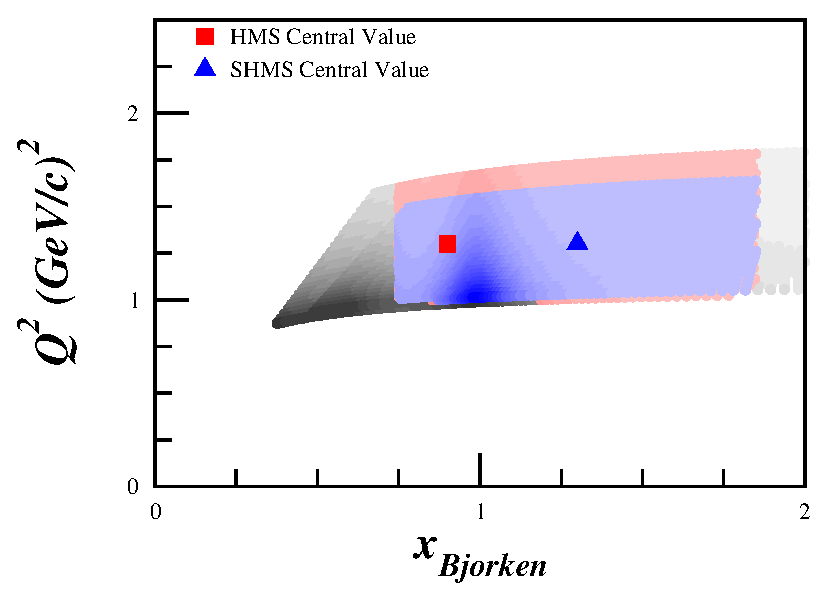
\includegraphics[width=0.49\textwidth]{figs/kine/Pzz_30_q2.eps}~~ %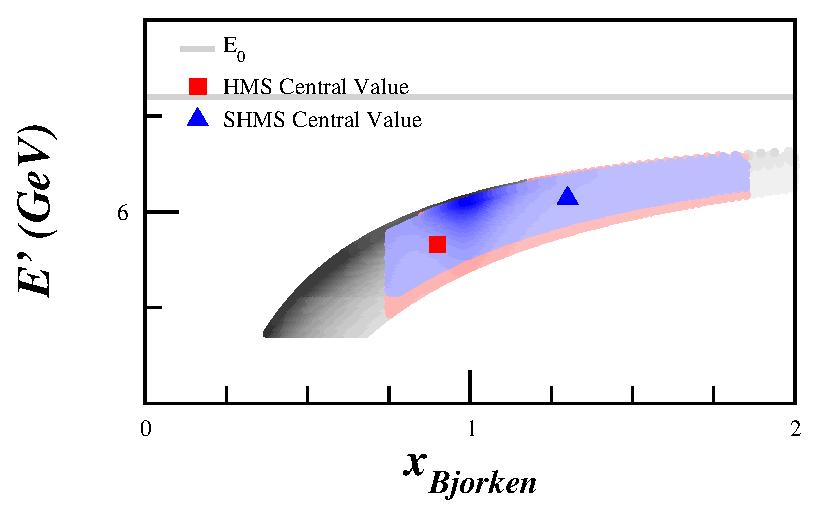
\includegraphics[width=0.49\textwidth]{figs/kine/Pzz_30_eprime.eps}
%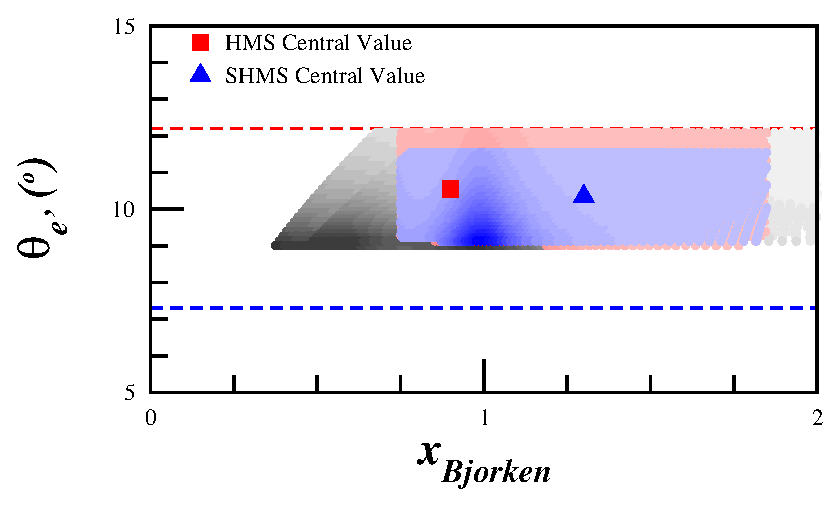
\includegraphics[width=0.49\textwidth]{figs/kine/Pzz_30_theta_eprime.eps}~~ 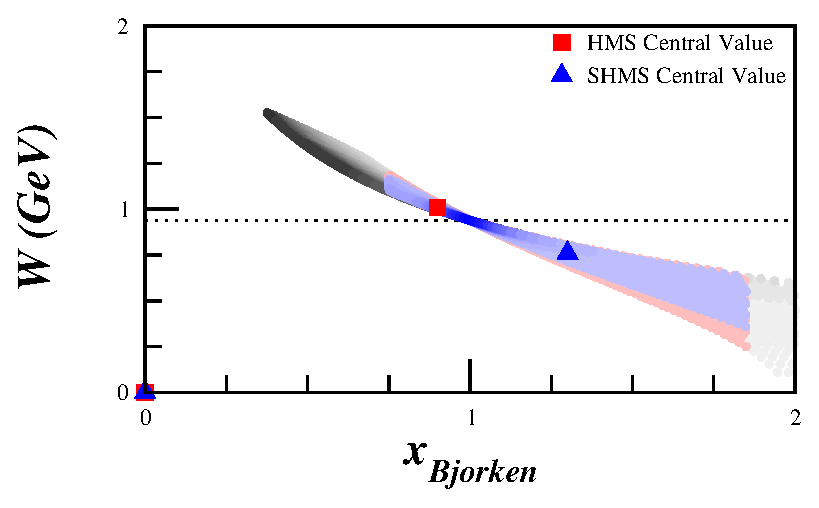
\includegraphics[width=0.49\textwidth]{figs/kine/Pzz_30_w.eps}
\caption{\label{kincov} Kinematic coverage.  The grey settings are not included in our rates estimates since they fall outside of $\XMIN < x < \XMAX$. The highlighted represent the central value of the spectrometer setting, which are not the statistics weighted average of the distribution. The shading represents areas with greater statistics.}
\end{center}
\end{figure}


The polarized \TARGET target is discussed in section~\ref{POLTARGSEC}.  The magnetic field of the target will be held constant along the beamline at all times, while the target state is alternated between a polarized and unpolarized state.
The tensor polarization and packing fraction used in the rates estimate are \PZZ\% and \PF, respectively. 
The packing fraction changes with $x$ in the range of this measurement as shown in Fig.~\ref{fdil_plot}.
With an incident
electron beam current of \CURRENT nA, the
expected deuteron luminosity is $1.57\times 10^{35}$ / cm$^2\cdot$s$^1$. The momentum bite and the acceptance
were assumed to be $\Delta P = \pm 8\%$ and $\Delta\Omega = 5.6$ msr for the HMS, and $\Delta P= ^{+20\%}_{-8\%}$ 
%$-8<\Delta P <+20\%$
and $\Delta\Omega =4.4$ msr for the SHMS. 
%
For the choice of the kinematics,
special attention was taken onto the angular and momentum limits of the spectrometers: for the
HMS, $10.5^{\circ} \le \theta \le 85^{\circ}$ and $1 \le P_0 \le 7.3$ GeV/c, and for the SHMS,
$5.5^{\circ} \le \theta \le 40^{\circ}$ and $2 \le P_0 \le 11$ GeV/c. In addition, the
opening angle between the spectrometers is physically constrained to be larger than 17.5$^{\circ}$.
The invariant mass $W$ was kept to $W \ge \WMIN$ GeV for all settings.
The projected 
uncertainties and $A_{zz}$
are summarized in Table~\ref{RATES2}, and displayed in
Fig.~\ref{PROJ}.  

\begin{figure}
\begin{center}
%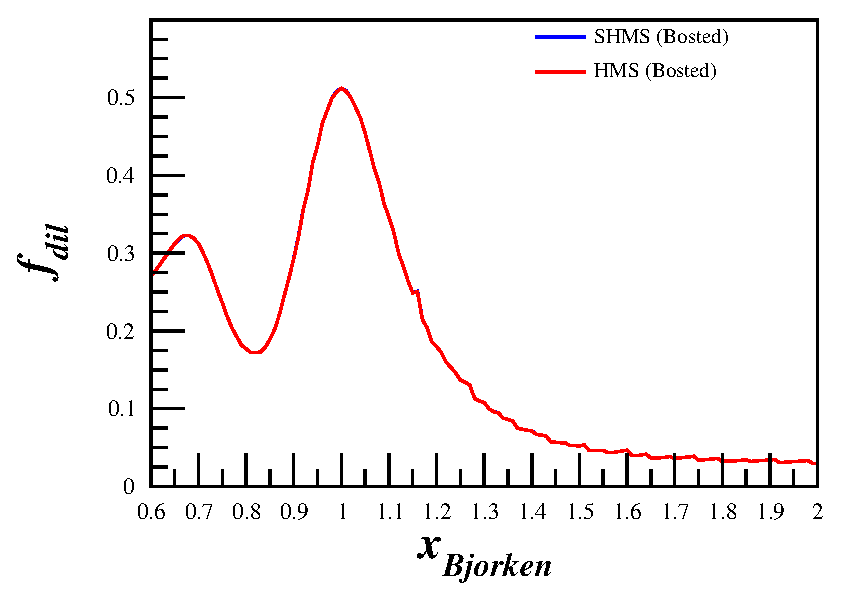
\includegraphics[width=0.5\textwidth]{figs/kine/Pzz_30_fdil.eps} 
\caption{\label{fdil_plot}Projected dilution fraction covering the entire $x$ range to be measured using the Bosted fits \cite{Bosted:2012qc} for the SHMS and HMS. In the kinematics used, both dilution factors overlap.}
\end{center}
\end{figure}

\begin{figure}
\begin{center}
%\includegraphics[width=0.45\textwidth]{figs/plots0705/b1_proj_newmiller_lin.eps}
%\hspace{0.5cm}
%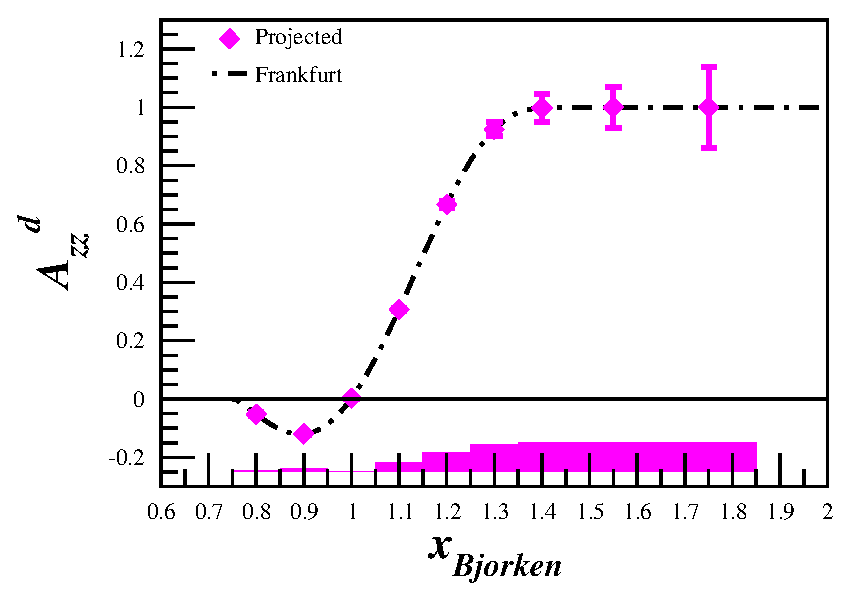
\includegraphics[width=0.5\textwidth]{figs/kine/Pzz_30_Azz_nobars.eps} 
\caption{\label{PROJ}Projected statistical errors for the tensor asymmetry $A_{zz}$ with \productiondays days of beam time. Data at different $Q^2$ are combined with an x-binning that varies slightly per point, but is approximately $\pm0.05$. The band represents the systematic uncertainty. Also shown are the calculations from Frankfurt and Strikman \cite{Frankfurt:1988nt}.
}
\end{center}
\end{figure}

A total of 
\productiondays
 days of beam time is requested for production data, with an additional \overheaddays days of expected overhead.



\clearpage

%





